% Preamble
\documentclass[11pt,pdf, aspectratio=169]{beamer}
\usetheme{metropolis}
\title{DAPC 2023 Training Sessions\\Session 3}
\author{Verwoerd}
\date{September 18, 2023}

% Packages
\usepackage{amsmath}
\usepackage[utf8]{inputenc}
\usepackage[T1]{fontenc}
\usepackage{graphicx}
\usepackage{tikz}
\usepackage{minted}
\usepackage[
  type={CC},
  modifier={by-sa},
  version={4.0},
]{doclicense}
\usepackage{hyperref}
\setsansfont{Fira Sans}
\usemintedstyle{manni}
\setminted{
  fontsize=\footnotesize,linenos,frame=lines, framesep=2mm
}
\usetikzlibrary{angles,quotes,graphs, graphdrawing,positioning}
\usegdlibrary {layered}

\begin{document}
  \maketitle
  \begin{frame}{Session 3}
    \begin{itemize}
      \item Team Reference Document
      \item Solutions to Sorting and Search Problems
      \item Solving interactive problems
      \item Solving Dynamic Programming Problems
    \end{itemize}
    Slides are available on \url{https://chipcie.wisv.ch/} in the training news post.
    \doclicenseThis
  \end{frame}


  \section{Team Reference Document}
  \begin{frame}{Team Reference Document}
    \begin{itemize}
      \item During the DAPC you may bring any analogue reference material you want
      \item Starting from the BAPC, you may only bring limited reference material
      (= same rules as World Finals)
      \item This reference is called the Team Reference Document (TRD)
      \item Sometimes the old term Team Contest Reference (TCR) is used
    \end{itemize}
  \end{frame}
  \begin{frame}{Team Reference Document: Rules}
    \begin{quote}
      Each contestant may bring an \emph{(identical)} copy of a Team Reference Document.
      This document may contain up to 25 pages of reference materials, single-sided, letter or A4 size, with pages numbered in the upper right-hand corner and your university name printed in the upper left-hand corner.
      Text and illustrations must be readable by a person with correctable eyesight without magnification from a distance of ½ meter.
      It may include handwritten comments and corrections on the fronts of pages only.
      The document should be in some type of notebook or folder with the name of your institution on the front.
    \end{quote}
  \end{frame}
  \begin{frame}{TRD: Example}
    \includegraphics[width=.8\linewidth]{images/session-3/tcr-1}
  \end{frame}
  \begin{frame}{TRD: Example}
    \includegraphics[width=.8\linewidth]{images/session-3/tcr-2}
  \end{frame}
  \begin{frame}{TRD: Example}
    \includegraphics[width=.8\linewidth]{images/session-3/tcr-3}
  \end{frame}
  \begin{frame}{TRD: Example}
    \includegraphics[width=.8\linewidth]{images/session-3/tcr-4}
  \end{frame}
  \begin{frame}{Potential subjects in a TRD}
    \begin{columns}
      \begin{column}{.45\textwidth}
        \begin{enumerate}
          \item Mathematics
          \begin{itemize}
            \item Formulas and Theories
            \item Trigonometry
          \end{itemize}
          \item Data Structures
          \begin{itemize}
            \item Segement Tree, Treap, RMQ
            \item HashMap, PriorityQueue
          \end{itemize}
          \item Numerical Methods
          \begin{itemize}
            \item Simplex, Integration
            \item Linear Problem-solving
          \end{itemize}
          \item Number Theory
          \begin{itemize}
            \item Primality, Divisability
          \end{itemize}
          \item Combinatorial
          \begin{itemize}
            \item Permutations, Partitions
          \end{itemize}
        \end{enumerate}
      \end{column}
      \begin{column}{.45\textwidth}
        \begin{enumerate}
          \addtocounter{enumi}{5}
          \item Graph
          \begin{itemize}
            \item Search algorithms
            \item Flow algorithms
            \item Spanning Tree, Connected Components
          \end{itemize}
          \item Geometry
          \begin{itemize}
            \item Line intersection, length
            \item Triangles and Circles
            \item Polygons
          \end{itemize}
          \item Strings
          \item Templates
          \item Tests and reminders
        \end{enumerate}
      \end{column}
    \end{columns}
  \end{frame}
  \begin{frame}{Tips on TRD}
    \begin{itemize}
      \item Only put stuff in that you know how/when to use
      \item Ensure that the code is correct and complete
      \item Add short description, complexity, and hash
      \item Evaluate document after each contest for improvements
      \item Several templates available at \texttt{https://chipcie.wisv.ch/resources}
    \end{itemize}
  \end{frame}


  \section{Solutions to the sorting and search problems}
  \begin{frame}{Abbreviated Aliases}
    \begin{itemize}
      \item Source BAPC Preliminaries 2022
      \item Time limit: 2s
      \item For every username calculate the size of the shortest unique prefix.
    \end{itemize}
    Original problem written by the BAPC 2022 jury and licensed under \doclicenseLongNameRef.

    \doclicenseImage
  \end{frame}

  \begin{frame}{Abbreviated Aliases}
    \begin{itemize}
      \item<+-> Observation: $n\cdot l \leq 10^7$, so we are aiming for $\mathcal{O}(n\log{}n)$
      \item<+-> Comparing every username with all other usernames is $\mathcal{O}(n^2)$, which is too slow
      \item<+-> We only need to compare the two usernames where the prefix is most similar\\
      \texttt{james} is closest to \texttt{jacob} and \texttt{janos}, there is no other username that will increase the prefix
      \item<+-> If we sort the list, we only have to compare with the username before and after
      \item<+-> Alternatively, build a compressed Trie, and for each leaf, count the distance to the root
    \end{itemize}
  \end{frame}
  \begin{frame}[containsverbatim]{Abbreviated Aliases}
    \inputminted{python}{code/session-1/python/dapc-a.py}
  \end{frame}

  \begin{frame}{Dimensional Debugging}
    \begin{itemize}
      \item Source BAPC Preliminaries 2022
      \item Time limit: 2s
      \item Given $n$ algorithms that only work when their input $\varphi$ is small enough ($\varphi \leq H$), can you verify the correctness on sufficient large inputs ($\varphi \geq L$).
    \end{itemize}
    Original problem written by the BAPC 2022 jury and licensed under \doclicenseLongNameRef.

    \doclicenseImage
  \end{frame}

  \begin{frame}{Dimensional Debugging}
    \begin{itemize}
      \item<+-> Observation: $n \leq 10^3$, so we are aiming for an $\mathcal{O}(n^2)$ algorithm.
      \item<+-> We can verify all algorithms with $L = \varphi_0$
      \item<+-> Add those algorithms to verified algorithms, then find any unverified where $H_j \leq L_i$
      \item<+-> In this way you can create a graph between the different algorithms.
      \item<+-> Use a flood fill by BFS/DFS to count the number of algorithms you can reach.
      \item<+-> This results in an $\mathcal{O}(n^2)$ algorithm.
    \end{itemize}
  \end{frame}
  \begin{frame}[containsverbatim]{Dimensional Debugging}
    \inputminted[fontsize=\tiny]{python}{code/session-1/python/dapc-d.py}
  \end{frame}

  \begin{frame}{Extended Braille}
    \begin{itemize}
      \item Source BAPC Preliminaries 2022
      \item Time limit: 8s
      \item Given $n$ braille characters by their points, determine how many of them are distinct up to translation.
    \end{itemize}
    Original problem written by the BAPC 2022 jury and licensed under \doclicenseLongNameRef.

    \doclicenseImage

  \end{frame}
  \begin{frame}{Extended Braille}
    \begin{itemize}
      \item<+-> Observation 1: time limit of 8s is due to high input size
      \item<+-> Observation 2: at most $10^6$ dots, so we are looking for $\mathcal{O}(n\log{}n)$
      \item<+-> Per Braille character, sort the dots on $x$ then $y$
      \item<+-> Move the first ordered dot to $(0, 0)$ by subtracting the first point coordinate from all the dots\\
      \quad$\forall_{i=1}^m (x'_i, y'_i) = (x_i - x_1, y_i - y_1)$
      \item<+-> Add the transposed characters to a HashMap or Set and count the unique keys
      \item<+-> Resulting a $\mathcal{O}(n\log{}n)$ or amortized $\mathcal{O}(n)$
    \end{itemize}
  \end{frame}
  \begin{frame}[containsverbatim]{Extended Braille}
    \inputminted{python}{code/session-1/python/dapc-e.py}
  \end{frame}
  \begin{frame}{Knitting Pattern}
    \begin{itemize}
      \item Source BAPC Preliminaries 2022
      \item Time limit: 3s
      \item Given a knitting pattern and amount of wool it costs for letting the wool strand unused, using the wool in a stitch, and for starting or ending the use of wool.
      Compute the minimal amount of wool required for every colour of wool.
    \end{itemize}
    Original problem written by the BAPC 2022 jury and licensed under \doclicenseLongNameRef.

    \doclicenseImage
  \end{frame}
  \begin{frame}{Knitting Pattern}
    \begin{itemize}
      \item<+-> Observation: $|p| \leq 10^6$, so we are aiming for a $\mathcal{O}(|p|\log{}|p|)$
      \item<+-> For gap between colours you have 2 options
      \begin{enumerate}
        \item<+-> let the strand continue
        \item<+-> stop the strand and start again
      \end{enumerate}
      \item<+-> For every colour, we have to calculate for every gap: \[\min(c_{stop}+c_{start}, gap_{size}\cdot c_{unused})\]
      \item<+-> Calculate the total cost for each colour and sum it together
      \item<+-> The complexity is $\mathcal{O}(|w|\cdot |p|)$, or in a single pass over $p$ with creative bookkeeping
    \end{itemize}
  \end{frame}
  \begin{frame}[containsverbatim]{Knitting Pattern}
    \inputminted{python}{code/session-1/python/dapc-k.py}
  \end{frame}

  \begin{frame}{Kiosk Construction}
    \begin{itemize}
      \item Source BAPC 2022
      \item Time limit: 8s
      \item Find the optimal kiosk position for a given camping layout.
    \end{itemize}
    Original problem written by the BAPC 2022 jury and licensed under \doclicenseLongNameRef.

    \doclicenseImage
  \end{frame}
  \begin{frame}{Kiosk Construction}
    \begin{itemize}
      \item<+-> The shortest path for every kiosk position to every other plot can be found by using DFS/BFS
      \item<+-> Then find the kiosk(s) that can reach all plot and minimize the maximum distance
      \item<+-> Doing $n^2$ DFS/BFS for every kiosk results in a $\mathcal{O}(n^3)$ solution and receives a TLE
      \item<+-> You an optimize do to some preprocessing, calculate the distance from every plot to every kiosk position, storing intermediate results
      \item<+-> This optimization results in a $\mathcal{O}(n^2)$ solution
    \end{itemize}
  \end{frame}
  \begin{frame}[containsverbatim]{Kiosk Construction}
    \inputminted[fontsize=\tiny]{python}{code/session-1/python/bapc-k.py}
  \end{frame}


  \section{Solving interactive problems}
  \begin{frame}{What are Interactive Problems?}
    \begin{itemize}
      \item Traditional problems give all the input at once, you solve and print all the output at once
      \item Interactive problems give input, you do work, print output, and you receive new input
      \item This process continues until you find the final answer
      \item The problem defines an interaction protocol
      \item The problem may have an interaction limit
      \item If an interactive problem may be in the set, an simple interactive problem will be included in the test session
    \end{itemize}
  \end{frame}
  \begin{frame}{Type of problems for Interactive Problems}
    \begin{itemize}
      \item Search in a finite space
      \item Explore a maze
      \item Matching games
      \item Double interaction problem (very, very rare)
      \begin{itemize}
        \item Program has 2 modes
        \item the first mode, input transforms input to output following certain rules
        \item The second mode, the output of mode 1 is given and you have tranform it back to the input of mode 1
      \end{itemize}
    \end{itemize}
  \end{frame}
  \begin{frame}{Common pitfalls for Interactive problems}
    \begin{itemize}
      \item Flush the output after every write
      \begin{itemize}
        \item Only the output, not the input
        \item Not flushing the output results in Time Limit Exceeded
      \end{itemize}
      \item Verdict of a solution is not deterministic, but the following is guaranteed:
      \begin{itemize}
        \item Wrong Answer means you printed something wrong
        \item Runtime Error means you returned an 0 error code
        \item If both occur, you will get either
      \end{itemize}
      \item ICPC style contests don't have ``Idleness Limit Exceeded'', but a total runtime limit.
    \end{itemize}
  \end{frame}
  \begin{frame}{Flushing the output}
    \begin{description}
      \item [C++]: end your output with \mintinline{c++}|std::endl| or \mintinline{c++}|std::flush|
      \item[Python]: use the flush parameter, like \mintinline{python}|print("abc", flush=True)|
      \item[Java/Kotlin]: use a \mintinline{java}|java.io.BufferedWriter| and after each write use the \mintinline{java}|.flush()| method.
    \end{description}
  \end{frame}
  \begin{frame}{Interactive problems testing tool}
    \begin{itemize}
      \item Most contests provide a testing tool to test the interaction with a testing tool
      \item This is usually called \texttt{testing\_tool.py} in our region
      \item The header file tells you how to run run the testing tool, for example\\\texttt{\textdollar{} python3 testing\_tool.py -f 1.in python3 ./solution.py}
      \item Pitfall for Java/Kotlin: You should run the testing tool in the directory which contains the compiled class file

      \item \textbf{Wrong}:\\\texttt{\textasciitilde/\textdollar{} python3 testing\_tool.py -f 1.in java ./code/ProblemA}
      \item \textbf{Right}:\\\texttt{\textasciitilde/code/\textdollar{} python3 testing\_tool.py -f 1.in java ProblemA}
    \end{itemize}
  \end{frame}
  \begin{frame}{Example Interactive Problem}
    You are asked to guess a number between 0 and $n$.
  \end{frame}
  \begin{frame}{Example Interactive Problem: Interaction}
    This is an interactive problem.
    Your submission will be run against an interactor, which reads from the standard output of your submission and writes to the standard input of your submission.
    This interaction needs to follow a specific protocol:

    The interactor first sends one line with an integer $n$ ($3 \leq n \leq 1000$), the upper bound of the guessing game.

    You can then send a guess $g$ ($0\leq g \leq n$).

    The interactor will respond with the strings \texttt{lower}, \texttt{higher}, or \texttt{correct}.
    This represents is if the number to guess is lower, higher, or correct, respectively.
    After you have guessed the correct number, you should exit the program.

    The interactor is not adaptive, i.e. the secret number is fixed during a round.
    Using more than $12$ guesses will result in a wrong answer.
  \end{frame}
  \begin{frame}{Example Interactive Problem: Example interaction}
    \begin{tabular}{|l|l|}
      \hline
      \textbf{Sample Input 1} & \textbf{Sample Output 1} \\
      \hline
      \texttt{1000}           &                          \\
      & \texttt{67}              \\
      \texttt{higher}         &                          \\
      & \texttt{967}             \\
      \texttt{lower}          &                          \\
      & \texttt{500}             \\
      \texttt{correct}        &                          \\
      \hline
    \end{tabular}
  \end{frame}

  \begin{frame}[containsverbatim]{Example Interactive Problem: Python Solution}
    \inputminted{python}{code/session-1/python/interactive-example.py}
  \end{frame}
  \begin{frame}[containsverbatim]{Example Interactive Problem: C++ Solution}
    \inputminted[fontsize=\tiny]{c++}{code/session-1/c++/interactive-example.cpp}
  \end{frame}
  \begin{frame}[containsverbatim]{Example Interactive Problem: Java Solution}
    \inputminted[fontsize=\tiny]{java}{code/session-1/java/InteractiveExample.java}
  \end{frame}
  \begin{frame}[containsverbatim]{Example Interactive Problem: Kotlin Solution}
    \inputminted{kotlin}{code/session-1/kotlin/interactive-example.kt}
  \end{frame}


  \section{Solving Dynamic Programming Problems}
  \begin{frame}{Dynamic Programming}
    \begin{itemize}
      \item Dynamic Programming (DP) is a techinque of solving problem by solving an problem by solving it in a recursive simpler sub-problem
      \item DP requires an overlap to occur, else its considered a Divide and Conquer algorithm
    \end{itemize}
  \end{frame}
  \begin{frame}[containsverbatim]{Dynamic Programming: Fibonacci Numbers}
    \begin{itemize}
      \item The formula is $\mathcal{F}_i = \mathcal{F}_{i-1} + \mathcal{F}_{i-2}$
      \item It depends clearly on previous calculations
      \item It can be solved by $\mathcal{F}_1$ and $\mathcal{F}_2$ which are both 1
    \end{itemize}
    \begin{minted}{python}
def fibonacci(n):
  if n == 1 or n == 2:
    return 1
  else:
    return fibonacci(n - 1) + fibonacci(n - 2)
    \end{minted}
    \begin{minted}{kotlin}
fun fibonacci(i: Long): Long = when(i) {
  1L, 2L -> 1
  else -> fibonacci(i - 1) + fibonacci(i - 2)
}
    \end{minted}
  \end{frame}
  \begin{frame}[containsverbatim]{Dynamic Programming: Fibonacci Numbers: Caching}
    \begin{minted}{python}
@lru_cache(None)
def fibonacci(n):
  if n == 1 or n == 2:
    return 1
  else:
    return fibonacci(n - 1) + fibonacci(n - 2)
    \end{minted}
    \begin{minted}{kotlin}
val cache = mutableMapOf<Long, Long>()
fun fibonacci(i: Long): Long = when(i) {
  1L, 2L -> 1
  else -> cache.getOrPut(i - 1) { fibonacci(i - 1) }
        + cache.getOrPut(i - 2) { fibonacci(i - 2) }
}
    \end{minted}
  \end{frame}
  \begin{frame}{Dynamic Programming: Using States}
    Consider a weighted graph with a adjacency matrix $w$
    \begin{columns}
      \column{.5\textwidth}
      \begin{tikzpicture}
        \graph[layered layout] {

          B --[edge label=5] C --[edge label=1] F;
          B --[edge label=5] D --[edge label=1] F;
          A --[edge label=1] E;
          A --[edge label=7] B --[edge label=1] E --[edge label=3] F;
        };
      \end{tikzpicture}
      \column{.5\textwidth}
      \[ w = \begin{bmatrix}
               0      & 7      & \infty & \infty & 1      & \infty \\
               7      & 0      & 5      & 5      & 1      & \infty \\
               \infty & 5      & 0      & \infty & \infty & 1      \\
               1      & 5      & \infty & 0      & \infty & 1      \\
               \infty & 1      & \infty & \infty & 0      & 3      \\
               \infty & \infty & 1      & 1      & 3      & 0
      \end{bmatrix}\]
    \end{columns}
    Calculate a matrix giving the shortest path from and to all nodes (All Pair Shortest Path (APSP)).
  \end{frame}
  \begin{frame}{Dynamic Programming: Using States (APSP) }
    \begin{itemize}
      \item Calculating Dijkstra for every node is very inefficient
      \item Create the sub-problem calculate APSP with a subset of the connections
      \item Define $k$ as the number of nodes to use
      \item Then do the DP by using the following formula:\\
      \[
        f(i, j, k) = \begin{cases}
                       w(i, j)  & \text{if } k = 0\\
                       \min(f(i,j, k-1), f(i, k, k-1)+f(k, j, k-1))
        \end{cases}
      \]
      \item The shortest path between $i$ and $j$ with using only the first $k$ nodes is the min of:
      \begin{itemize}
        \item the shortest path when using $k-1$
        \item the shortest path from $i$ to $k$ plus the shortest path from $k$ to $j$
      \end{itemize}
      \item This is Floyd-Warshall's APSP with a complexity $\mathcal{O}(n^3)$
    \end{itemize}
  \end{frame}


  \section{Conclusion}
  \begin{frame}{Guest speaker}
    \textbf{Maarten Sijm}
    \begin{columns}
      \column{0.7\textwidth}
      \begin{itemize}
        \item Head of jury for BAPC since 2022
        \begin{itemize}
          \item FPC jury member since 2018
          \item BAPC jury member since 2020
          \item NWERC jury member since 2022
        \end{itemize}
        \item BAPC/NWERC particpant (best result: 24th)
        \begin{itemize}
          \item 2016: ``Tie Limit Exceeded''
          \item 2017: ``class RubberDuck extends Throwable \{\}''
          \item 2018: ``$\Omega(\raisebox{1.5ex-\height}{
\includegraphics[width=1em]{images/session-3/duck-emoji.png}}^n)$''
        \end{itemize}
        \item BSc+MSc Computer Science @ TU Delft
        \item Second-oldest member of CHipCie
      \end{itemize}
      \column{0.2\textwidth}
      \begin{center}
        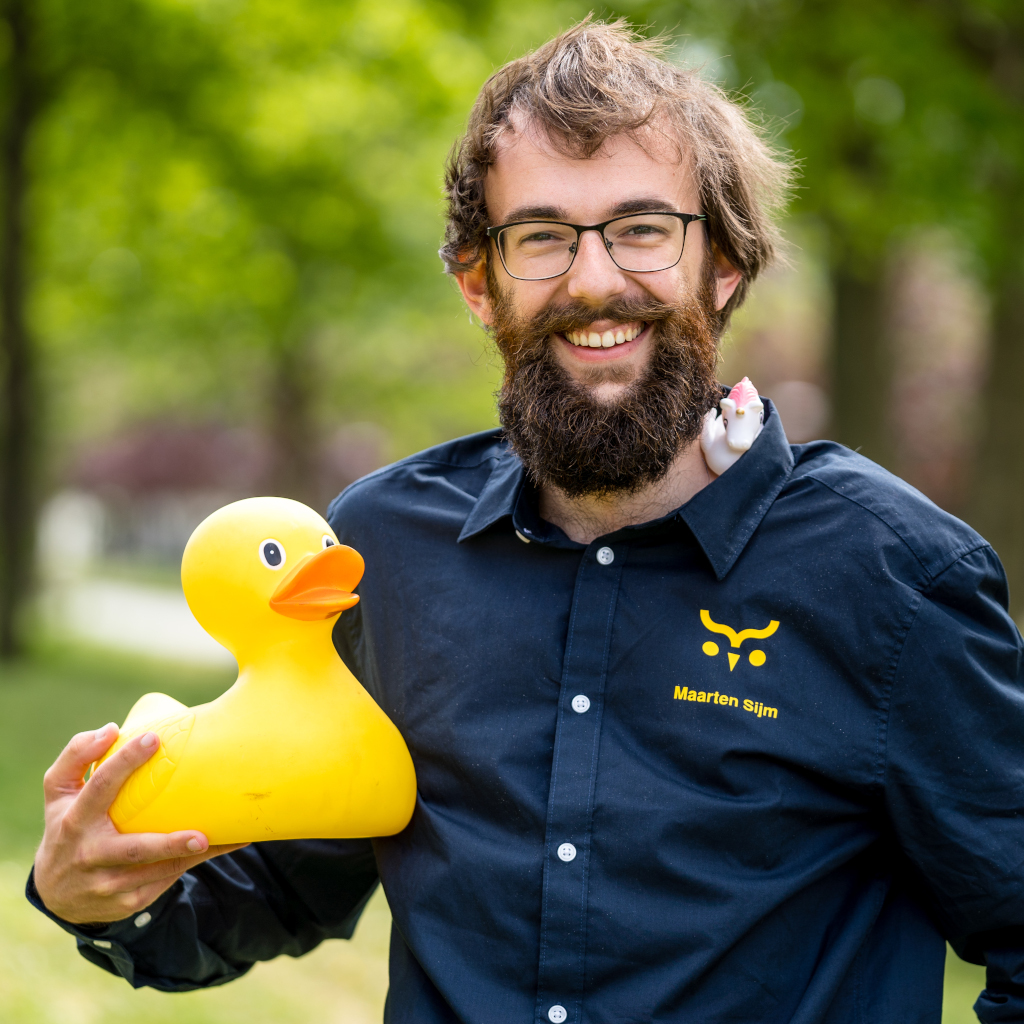
\includegraphics[width=\columnwidth]{images/session-3/jury-maarten.jpg}
      \end{center}
    \end{columns}
  \end{frame}
  \newcommand{\jurytimeline}[1]{
  %\vskip 0pt plus 1filll minus 0pt
    \vfill
    \vfill
    \begin{tikzpicture}[scale=0.138]
      \draw[line width=5,color=blue!50] (0,0) -- (60,0);
      \draw[line width=5,color=green!50] (60,0) -- (90,0);
      \draw[line width=5,color=blue!50] (90,0) -- (100,0);
      \node at (#1,0) {
\includegraphics[width=2em]{images/session-3/rubber-duck.png}};
    \end{tikzpicture}
    \vskip 0pt plus -1fill
  }
  \begin{frame}{Recipe for a Contest}
    \begin{itemize}
      \item About a dozen jury members
      \item Tens of problem ideas
      \item A few months of time
      \begin{itemize}
        \item Meeting every two weeks
      \end{itemize}
    \end{itemize}
    \jurytimeline{5}
  \end{frame}
  \begin{frame}{Problem Selection}
    \begin{itemize}
      \item Label problems submitted to Call for Problems
      \begin{itemize}
        \item How much we like the problem
        \item Difficulty rating
        \item Categories (math, geometry, graph, \dots)
      \end{itemize}
      \item Select problems that we like best, \\
      \quad{}with spread in difficulty and categories
    \end{itemize}
    \jurytimeline{15}
  \end{frame}
  \begin{frame}{Problem Naming}
    \begin{center}
      \parbox[c][0.55\textheight]{\textwidth}{%
        \includegraphics<+>[width=0.9\textwidth]{images/session-3/naming-sheet-1.png}%
        \includegraphics<+>[width=0.9\textwidth]{images/session-3/naming-sheet-2.png}%
      }%
      \\\small\emph{Problem naming sheet of DAPC 2022}
    \end{center}
    \jurytimeline{25}
  \end{frame}
  \begin{frame}{Problem Implementation}
    \begin{itemize}
      \item Problem statement (LaTeX)
      \item Generating test data (YAML spec + C++/Python scripts)
      \item Validating input (C++/Python scripts)
      \item Validating output (C++/Python scripts)
      \item Submissions in all supported languages
      \item Solution slides (LaTeX) \\[1em]
      \item Tooling: \url{github.com/RagnarGrootKoerkamp/BAPCtools}
    \end{itemize}
    \jurytimeline{35}
  \end{frame}
  \begin{frame}{Trying to Break Stuff}
    \begin{itemize}
      \item Constraints checking
      \begin{itemize}
        \item Minimal/maximal input
      \end{itemize}
      \item Fuzzing
      \begin{itemize}
        \item Generate more random test data from existing scripts
      \end{itemize}
      \item Write submissions that should be wrong/too slow
      \item Invite proof readers/solvers
    \end{itemize}
    \jurytimeline{45}
  \end{frame}
  \begin{frame}{Check That Everything Works}
    \begin{itemize}
      \item Continuous Integration
      \item Upload problems to DOMjudge
      \begin{itemize}
        \item Local machine
        \item Test in Drebbelweg with Maarten (systems Maarten)
      \end{itemize}
      \item Check time limits on contest hardware
    \end{itemize}
    \jurytimeline{55}
  \end{frame}
  \begin{frame}{Start of the Contest}
    \begin{itemize}
      \item Waiting for the first submissions to come in
      \item Taking guesses
      \begin{itemize}
        \item Which problem would be solved first, and after how many minutes?
        \item What will be the order of most-solved to least-solved?
      \end{itemize}
    \end{itemize}
    \jurytimeline{60}
  \end{frame}
  \begin{frame}{During the Contest}
    \begin{itemize}
      \item Check incoming submissions
      \begin{itemize}
        \item Are they correctly marked as AC/TLE/WA/\dots?
        \item Are they using clever solutions that we didn't think of?
      \end{itemize}
      \item Answer incoming clarification requests
      \begin{itemize}
        \item The dreadful ``\emph{No comment.}'' and \\
        ``\emph{Please read the problem statement carefully.}''
      \end{itemize}
      \item Add common mistakes to solution slides
    \end{itemize}
    \jurytimeline{75}
  \end{frame}
  \begin{frame}{During the Contest}
    \begin{center}
      \includegraphics<+>[width=\textwidth]{images/session-3/submissions-queue.png}
      \includegraphics<+>[height=0.8\textheight]{images/session-3/clarification-canned.png}
      \includegraphics<+>[height=0.8\textheight]{images/session-3/clarification-all.png}
    \end{center}
  \end{frame}
  \begin{frame}{After the Contest}
    \begin{itemize}
      \item Generate solve stats \\[0.5em]
      
\includegraphics[width=0.8\textwidth]{images/session-3/solve-stats.png}
      \item Present solutions
    \end{itemize}

    \vspace{2em}
    And, next year\dots

    \begin{itemize}
      \item Do it all over again!
    \end{itemize}
    \jurytimeline{95}
  \end{frame}

  \begin{frame}{Next Session}
    Next session is on Thursday the 21st of September.\\
    Guest Speaker: Jeroen op de Beek and Leon van der Waal from Segment goes BRRRR about geometry problems.

    \url{https://domjudge.ewi.tudelft.nl/}
  \end{frame}
\end{document}
